\section{Data}
\label{sec:data}
The data were collected from the Hacker One website

from 35 public bounty programs, we collected the awards received by security researchers, with their timestamps and rewards in dollars.

{\bf [insert a summary figure or table]}




Here, we consider the {\it time of discovery} when the reward is bestowed to the researcher (with its associated reward).



\begin{figure}
\begin{center}
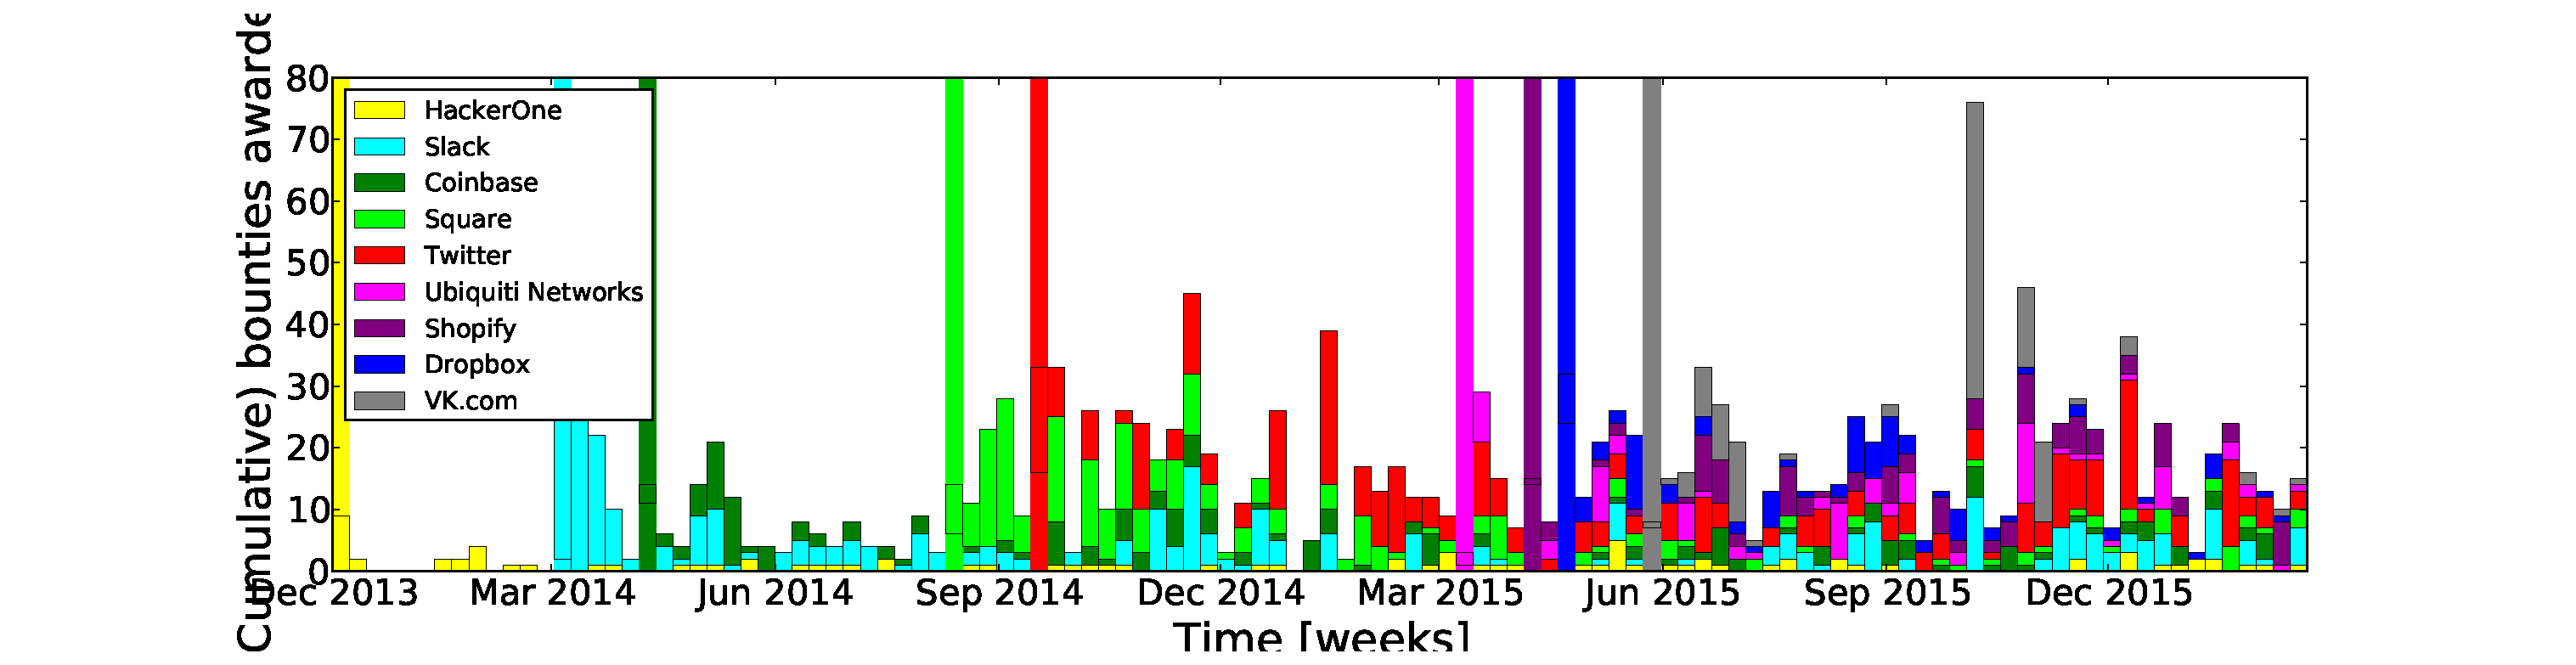
\includegraphics[width=17cm]{figures/timeline.eps}
\caption{{\bf A.} Weekly vulnerability discoveries for the 9 most active programs (with at least 90 bug discoveries as of Feb. 15, February). The light colored vertical bars represent the start of the program, occurring when the first bounty award. Most programs exhibit an initial shock (or shortly after the start of the program), followed by a decay of discoveries, which is characterized at the aggregate level by a long-memory process (panel {\bf B}) characterized by a power law decay $\sim t^{-0.34()}$ as shown on panel  (for all 35 public programs considered in this study).}
\label{ }
\end{center}
\end{figure}





